% Options for packages loaded elsewhere
\PassOptionsToPackage{unicode}{hyperref}
\PassOptionsToPackage{hyphens}{url}
%
\documentclass[
]{article}
\usepackage{amsmath,amssymb}
\usepackage{lmodern}
\usepackage{iftex}
\ifPDFTeX
  \usepackage[T1]{fontenc}
  \usepackage[utf8]{inputenc}
  \usepackage{textcomp} % provide euro and other symbols
\else % if luatex or xetex
  \usepackage{unicode-math}
  \defaultfontfeatures{Scale=MatchLowercase}
  \defaultfontfeatures[\rmfamily]{Ligatures=TeX,Scale=1}
\fi
% Use upquote if available, for straight quotes in verbatim environments
\IfFileExists{upquote.sty}{\usepackage{upquote}}{}
\IfFileExists{microtype.sty}{% use microtype if available
  \usepackage[]{microtype}
  \UseMicrotypeSet[protrusion]{basicmath} % disable protrusion for tt fonts
}{}
\makeatletter
\@ifundefined{KOMAClassName}{% if non-KOMA class
  \IfFileExists{parskip.sty}{%
    \usepackage{parskip}
  }{% else
    \setlength{\parindent}{0pt}
    \setlength{\parskip}{6pt plus 2pt minus 1pt}}
}{% if KOMA class
  \KOMAoptions{parskip=half}}
\makeatother
\usepackage{xcolor}
\usepackage[margin=1in]{geometry}
\usepackage{color}
\usepackage{fancyvrb}
\newcommand{\VerbBar}{|}
\newcommand{\VERB}{\Verb[commandchars=\\\{\}]}
\DefineVerbatimEnvironment{Highlighting}{Verbatim}{commandchars=\\\{\}}
% Add ',fontsize=\small' for more characters per line
\usepackage{framed}
\definecolor{shadecolor}{RGB}{248,248,248}
\newenvironment{Shaded}{\begin{snugshade}}{\end{snugshade}}
\newcommand{\AlertTok}[1]{\textcolor[rgb]{0.94,0.16,0.16}{#1}}
\newcommand{\AnnotationTok}[1]{\textcolor[rgb]{0.56,0.35,0.01}{\textbf{\textit{#1}}}}
\newcommand{\AttributeTok}[1]{\textcolor[rgb]{0.77,0.63,0.00}{#1}}
\newcommand{\BaseNTok}[1]{\textcolor[rgb]{0.00,0.00,0.81}{#1}}
\newcommand{\BuiltInTok}[1]{#1}
\newcommand{\CharTok}[1]{\textcolor[rgb]{0.31,0.60,0.02}{#1}}
\newcommand{\CommentTok}[1]{\textcolor[rgb]{0.56,0.35,0.01}{\textit{#1}}}
\newcommand{\CommentVarTok}[1]{\textcolor[rgb]{0.56,0.35,0.01}{\textbf{\textit{#1}}}}
\newcommand{\ConstantTok}[1]{\textcolor[rgb]{0.00,0.00,0.00}{#1}}
\newcommand{\ControlFlowTok}[1]{\textcolor[rgb]{0.13,0.29,0.53}{\textbf{#1}}}
\newcommand{\DataTypeTok}[1]{\textcolor[rgb]{0.13,0.29,0.53}{#1}}
\newcommand{\DecValTok}[1]{\textcolor[rgb]{0.00,0.00,0.81}{#1}}
\newcommand{\DocumentationTok}[1]{\textcolor[rgb]{0.56,0.35,0.01}{\textbf{\textit{#1}}}}
\newcommand{\ErrorTok}[1]{\textcolor[rgb]{0.64,0.00,0.00}{\textbf{#1}}}
\newcommand{\ExtensionTok}[1]{#1}
\newcommand{\FloatTok}[1]{\textcolor[rgb]{0.00,0.00,0.81}{#1}}
\newcommand{\FunctionTok}[1]{\textcolor[rgb]{0.00,0.00,0.00}{#1}}
\newcommand{\ImportTok}[1]{#1}
\newcommand{\InformationTok}[1]{\textcolor[rgb]{0.56,0.35,0.01}{\textbf{\textit{#1}}}}
\newcommand{\KeywordTok}[1]{\textcolor[rgb]{0.13,0.29,0.53}{\textbf{#1}}}
\newcommand{\NormalTok}[1]{#1}
\newcommand{\OperatorTok}[1]{\textcolor[rgb]{0.81,0.36,0.00}{\textbf{#1}}}
\newcommand{\OtherTok}[1]{\textcolor[rgb]{0.56,0.35,0.01}{#1}}
\newcommand{\PreprocessorTok}[1]{\textcolor[rgb]{0.56,0.35,0.01}{\textit{#1}}}
\newcommand{\RegionMarkerTok}[1]{#1}
\newcommand{\SpecialCharTok}[1]{\textcolor[rgb]{0.00,0.00,0.00}{#1}}
\newcommand{\SpecialStringTok}[1]{\textcolor[rgb]{0.31,0.60,0.02}{#1}}
\newcommand{\StringTok}[1]{\textcolor[rgb]{0.31,0.60,0.02}{#1}}
\newcommand{\VariableTok}[1]{\textcolor[rgb]{0.00,0.00,0.00}{#1}}
\newcommand{\VerbatimStringTok}[1]{\textcolor[rgb]{0.31,0.60,0.02}{#1}}
\newcommand{\WarningTok}[1]{\textcolor[rgb]{0.56,0.35,0.01}{\textbf{\textit{#1}}}}
\usepackage{longtable,booktabs,array}
\usepackage{calc} % for calculating minipage widths
% Correct order of tables after \paragraph or \subparagraph
\usepackage{etoolbox}
\makeatletter
\patchcmd\longtable{\par}{\if@noskipsec\mbox{}\fi\par}{}{}
\makeatother
% Allow footnotes in longtable head/foot
\IfFileExists{footnotehyper.sty}{\usepackage{footnotehyper}}{\usepackage{footnote}}
\makesavenoteenv{longtable}
\usepackage{graphicx}
\makeatletter
\def\maxwidth{\ifdim\Gin@nat@width>\linewidth\linewidth\else\Gin@nat@width\fi}
\def\maxheight{\ifdim\Gin@nat@height>\textheight\textheight\else\Gin@nat@height\fi}
\makeatother
% Scale images if necessary, so that they will not overflow the page
% margins by default, and it is still possible to overwrite the defaults
% using explicit options in \includegraphics[width, height, ...]{}
\setkeys{Gin}{width=\maxwidth,height=\maxheight,keepaspectratio}
% Set default figure placement to htbp
\makeatletter
\def\fps@figure{htbp}
\makeatother
\setlength{\emergencystretch}{3em} % prevent overfull lines
\providecommand{\tightlist}{%
  \setlength{\itemsep}{0pt}\setlength{\parskip}{0pt}}
\setcounter{secnumdepth}{-\maxdimen} % remove section numbering
\ifLuaTeX
  \usepackage{selnolig}  % disable illegal ligatures
\fi
\IfFileExists{bookmark.sty}{\usepackage{bookmark}}{\usepackage{hyperref}}
\IfFileExists{xurl.sty}{\usepackage{xurl}}{} % add URL line breaks if available
\urlstyle{same} % disable monospaced font for URLs
\hypersetup{
  pdftitle={Bayesian Linear Analysis},
  pdfauthor={Megan Feddern},
  hidelinks,
  pdfcreator={LaTeX via pandoc}}

\title{Bayesian Linear Analysis}
\author{Megan Feddern}
\date{2023-04-28}

\begin{document}
\maketitle

Mapping Bakun Index locations

\begin{Shaded}
\begin{Highlighting}[]
\NormalTok{map}
\end{Highlighting}
\end{Shaded}

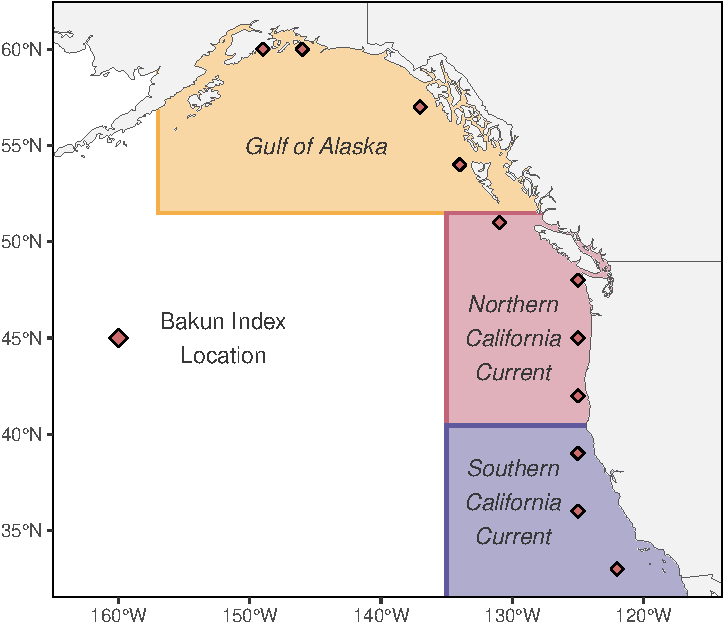
\includegraphics{BayesianLinearModels_files/figure-latex/map2-1.pdf}

\hypertarget{combining-bakun-data}{%
\subsection{Combining Bakun Data}\label{combining-bakun-data}}

\begin{enumerate}
\def\labelenumi{\arabic{enumi})}
\item
  Import the Bakun upwelling data from each individual file associated
  with the 13 lat/long locations. Data versions are: 1˚ 6-hourly version
\item
  Extract yyyy-mm-ddThh:mm:ss from the `time' column and add region
  indicator based on station ID and add a time period based on year
\item
  Summarize across days and hours to get monthly means for region and
  year. If you revert to seasonal summaries return to here to summarise
  across dates without taking means of means. Adding standardized
  upwelling index
\item
  Import PDO data, standardize across teh 1967 - 2022 time period
\end{enumerate}

\begin{enumerate}
\def\labelenumi{\Alph{enumi})}
\setcounter{enumi}{23}
\tightlist
\item
  Merging the standardized datasets into a single dataframe
\end{enumerate}

Run the STAN model outside of markdown file using ``STANrun.R'' which
exports the posteriors so that the model does not run in markdown when
you knit.

\hypertarget{stan-model}{%
\subsection{STAN Model}\label{stan-model}}

Bayesian linear model with era specific intercept and slope and region
specific slope,

\[Upwelling = \alpha_{e,r} + \beta_{e,r}*PDO +\sigma\] where \emph{e} is
factor ``era'' corresponding to eras 1967 - 1988, 1989 - 2013, and 2014
- 2022 and \emph{r} corresponds to regions Southern California Current
(south of Mendocino), Northern California Current (Mendocino to
Vancouver Island), and Gulf of Alaska (north of Vancover Island).

\begin{longtable}[]{@{}
  >{\raggedright\arraybackslash}p{(\columnwidth - 4\tabcolsep) * \real{0.2857}}
  >{\centering\arraybackslash}p{(\columnwidth - 4\tabcolsep) * \real{0.4286}}
  >{\raggedleft\arraybackslash}p{(\columnwidth - 4\tabcolsep) * \real{0.2857}}@{}}
\toprule()
\begin{minipage}[b]{\linewidth}\raggedright
Parameter
\end{minipage} & \begin{minipage}[b]{\linewidth}\centering
Description
\end{minipage} & \begin{minipage}[b]{\linewidth}\raggedleft
Prior
\end{minipage} \\
\midrule()
\endhead
\(\alpha_{e,r}\) & Era and region specific anomaly &
\(~ Normal(0,10)\) \\
\(\beta_{e,r}\) & Upwelling-PDO relationship by era and region &
\(~ Normal(0,10)\) \\
\(\sigma\) & Combined observation and process error &
\(~ Normal(0,10)[0,]\) \\
\bottomrule()
\end{longtable}

\hypertarget{monthly-mean-model}{%
\subsection{Monthly Mean Model}\label{monthly-mean-model}}

Linear relationship between monthly PDO Index and monthly upwelling
(Bakun 1˚ 6-hourly) for each era and each region estimated from a
Bayesian regression model.

\begin{verbatim}
## New names:
## `geom_smooth()` using formula = 'y ~ x'
## * `` -> `...1`
\end{verbatim}

\begin{verbatim}
## Warning in grid.Call(C_textBounds, as.graphicsAnnot(x$label), x$x, x$y, :
## conversion failure on 'Upwelling (Bakun 1˚ 6-hourly)' in 'mbcsToSbcs': dot
## substituted for <cb>
\end{verbatim}

\begin{verbatim}
## Warning in grid.Call(C_textBounds, as.graphicsAnnot(x$label), x$x, x$y, :
## conversion failure on 'Upwelling (Bakun 1˚ 6-hourly)' in 'mbcsToSbcs': dot
## substituted for <9a>
\end{verbatim}

\begin{verbatim}
## Warning in grid.Call(C_textBounds, as.graphicsAnnot(x$label), x$x, x$y, :
## conversion failure on 'Upwelling (Bakun 1˚ 6-hourly)' in 'mbcsToSbcs': dot
## substituted for <cb>
\end{verbatim}

\begin{verbatim}
## Warning in grid.Call(C_textBounds, as.graphicsAnnot(x$label), x$x, x$y, :
## conversion failure on 'Upwelling (Bakun 1˚ 6-hourly)' in 'mbcsToSbcs': dot
## substituted for <9a>
\end{verbatim}

\begin{verbatim}
## Warning in grid.Call(C_textBounds, as.graphicsAnnot(x$label), x$x, x$y, :
## conversion failure on 'Upwelling (Bakun 1˚ 6-hourly)' in 'mbcsToSbcs': dot
## substituted for <cb>
\end{verbatim}

\begin{verbatim}
## Warning in grid.Call(C_textBounds, as.graphicsAnnot(x$label), x$x, x$y, :
## conversion failure on 'Upwelling (Bakun 1˚ 6-hourly)' in 'mbcsToSbcs': dot
## substituted for <9a>
\end{verbatim}

\begin{verbatim}
## Warning in grid.Call(C_textBounds, as.graphicsAnnot(x$label), x$x, x$y, :
## conversion failure on 'Upwelling (Bakun 1˚ 6-hourly)' in 'mbcsToSbcs': dot
## substituted for <cb>
\end{verbatim}

\begin{verbatim}
## Warning in grid.Call(C_textBounds, as.graphicsAnnot(x$label), x$x, x$y, :
## conversion failure on 'Upwelling (Bakun 1˚ 6-hourly)' in 'mbcsToSbcs': dot
## substituted for <9a>
\end{verbatim}

\begin{verbatim}
## Warning in grid.Call(C_textBounds, as.graphicsAnnot(x$label), x$x, x$y, :
## conversion failure on 'Upwelling (Bakun 1˚ 6-hourly)' in 'mbcsToSbcs': dot
## substituted for <cb>
\end{verbatim}

\begin{verbatim}
## Warning in grid.Call(C_textBounds, as.graphicsAnnot(x$label), x$x, x$y, :
## conversion failure on 'Upwelling (Bakun 1˚ 6-hourly)' in 'mbcsToSbcs': dot
## substituted for <9a>
\end{verbatim}

\begin{verbatim}
## Warning in grid.Call(C_textBounds, as.graphicsAnnot(x$label), x$x, x$y, :
## conversion failure on 'Upwelling (Bakun 1˚ 6-hourly)' in 'mbcsToSbcs': dot
## substituted for <cb>
\end{verbatim}

\begin{verbatim}
## Warning in grid.Call(C_textBounds, as.graphicsAnnot(x$label), x$x, x$y, :
## conversion failure on 'Upwelling (Bakun 1˚ 6-hourly)' in 'mbcsToSbcs': dot
## substituted for <9a>
\end{verbatim}

\begin{verbatim}
## Warning in grid.Call(C_textBounds, as.graphicsAnnot(x$label), x$x, x$y, :
## conversion failure on 'Upwelling (Bakun 1˚ 6-hourly)' in 'mbcsToSbcs': dot
## substituted for <cb>
\end{verbatim}

\begin{verbatim}
## Warning in grid.Call(C_textBounds, as.graphicsAnnot(x$label), x$x, x$y, :
## conversion failure on 'Upwelling (Bakun 1˚ 6-hourly)' in 'mbcsToSbcs': dot
## substituted for <9a>
\end{verbatim}

\begin{verbatim}
## Warning in grid.Call.graphics(C_text, as.graphicsAnnot(x$label), x$x, x$y, :
## conversion failure on 'Upwelling (Bakun 1˚ 6-hourly)' in 'mbcsToSbcs': dot
## substituted for <cb>
\end{verbatim}

\begin{verbatim}
## Warning in grid.Call.graphics(C_text, as.graphicsAnnot(x$label), x$x, x$y, :
## conversion failure on 'Upwelling (Bakun 1˚ 6-hourly)' in 'mbcsToSbcs': dot
## substituted for <9a>
\end{verbatim}

\includegraphics{BayesianLinearModels_files/figure-latex/linearpdo-1.pdf}

Era specific intercepts across the entire region (Southern California
Current to Gulf of Alaska) estimated from a Bayesian regression model

\includegraphics{BayesianLinearModels_files/figure-latex/intercept-1.pdf}

\hypertarget{winter-model-nov---march}{%
\subsection{Winter Model (Nov - March)}\label{winter-model-nov---march}}

Using monthly mean data through winter months (Nov - Mar) where data is
standardized for the time period and season

Linear relationship between monthly PDO Index and monthly upwelling
(Bakun 1˚ 6-hourly) for each era and each region estimated from a
Bayesian regression model using Winter Monthly Means (Nov-March).

\begin{verbatim}
## New names:
## `geom_smooth()` using formula = 'y ~ x'
## * `` -> `...1`
\end{verbatim}

\begin{verbatim}
## Warning in grid.Call(C_textBounds, as.graphicsAnnot(x$label), x$x, x$y, :
## conversion failure on 'Upwelling (Bakun 1˚ 6-hourly)' in 'mbcsToSbcs': dot
## substituted for <cb>
\end{verbatim}

\begin{verbatim}
## Warning in grid.Call(C_textBounds, as.graphicsAnnot(x$label), x$x, x$y, :
## conversion failure on 'Upwelling (Bakun 1˚ 6-hourly)' in 'mbcsToSbcs': dot
## substituted for <9a>
\end{verbatim}

\begin{verbatim}
## Warning in grid.Call(C_textBounds, as.graphicsAnnot(x$label), x$x, x$y, :
## conversion failure on 'Upwelling (Bakun 1˚ 6-hourly)' in 'mbcsToSbcs': dot
## substituted for <cb>
\end{verbatim}

\begin{verbatim}
## Warning in grid.Call(C_textBounds, as.graphicsAnnot(x$label), x$x, x$y, :
## conversion failure on 'Upwelling (Bakun 1˚ 6-hourly)' in 'mbcsToSbcs': dot
## substituted for <9a>
\end{verbatim}

\begin{verbatim}
## Warning in grid.Call(C_textBounds, as.graphicsAnnot(x$label), x$x, x$y, :
## conversion failure on 'Upwelling (Bakun 1˚ 6-hourly)' in 'mbcsToSbcs': dot
## substituted for <cb>
\end{verbatim}

\begin{verbatim}
## Warning in grid.Call(C_textBounds, as.graphicsAnnot(x$label), x$x, x$y, :
## conversion failure on 'Upwelling (Bakun 1˚ 6-hourly)' in 'mbcsToSbcs': dot
## substituted for <9a>
\end{verbatim}

\begin{verbatim}
## Warning in grid.Call(C_textBounds, as.graphicsAnnot(x$label), x$x, x$y, :
## conversion failure on 'Upwelling (Bakun 1˚ 6-hourly)' in 'mbcsToSbcs': dot
## substituted for <cb>
\end{verbatim}

\begin{verbatim}
## Warning in grid.Call(C_textBounds, as.graphicsAnnot(x$label), x$x, x$y, :
## conversion failure on 'Upwelling (Bakun 1˚ 6-hourly)' in 'mbcsToSbcs': dot
## substituted for <9a>
\end{verbatim}

\begin{verbatim}
## Warning in grid.Call(C_textBounds, as.graphicsAnnot(x$label), x$x, x$y, :
## conversion failure on 'Upwelling (Bakun 1˚ 6-hourly)' in 'mbcsToSbcs': dot
## substituted for <cb>
\end{verbatim}

\begin{verbatim}
## Warning in grid.Call(C_textBounds, as.graphicsAnnot(x$label), x$x, x$y, :
## conversion failure on 'Upwelling (Bakun 1˚ 6-hourly)' in 'mbcsToSbcs': dot
## substituted for <9a>
\end{verbatim}

\begin{verbatim}
## Warning in grid.Call(C_textBounds, as.graphicsAnnot(x$label), x$x, x$y, :
## conversion failure on 'Upwelling (Bakun 1˚ 6-hourly)' in 'mbcsToSbcs': dot
## substituted for <cb>
\end{verbatim}

\begin{verbatim}
## Warning in grid.Call(C_textBounds, as.graphicsAnnot(x$label), x$x, x$y, :
## conversion failure on 'Upwelling (Bakun 1˚ 6-hourly)' in 'mbcsToSbcs': dot
## substituted for <9a>
\end{verbatim}

\begin{verbatim}
## Warning in grid.Call(C_textBounds, as.graphicsAnnot(x$label), x$x, x$y, :
## conversion failure on 'Upwelling (Bakun 1˚ 6-hourly)' in 'mbcsToSbcs': dot
## substituted for <cb>
\end{verbatim}

\begin{verbatim}
## Warning in grid.Call(C_textBounds, as.graphicsAnnot(x$label), x$x, x$y, :
## conversion failure on 'Upwelling (Bakun 1˚ 6-hourly)' in 'mbcsToSbcs': dot
## substituted for <9a>
\end{verbatim}

\begin{verbatim}
## Warning in grid.Call.graphics(C_text, as.graphicsAnnot(x$label), x$x, x$y, :
## conversion failure on 'Upwelling (Bakun 1˚ 6-hourly)' in 'mbcsToSbcs': dot
## substituted for <cb>
\end{verbatim}

\begin{verbatim}
## Warning in grid.Call.graphics(C_text, as.graphicsAnnot(x$label), x$x, x$y, :
## conversion failure on 'Upwelling (Bakun 1˚ 6-hourly)' in 'mbcsToSbcs': dot
## substituted for <9a>
\end{verbatim}

\includegraphics{BayesianLinearModels_files/figure-latex/linearpdoWINTER-1.pdf}

Era specific intercepts across the entire region (Southern California
Current to Gulf of Alaska) estimated from a Bayesian regression model
for winter months (Nov - March)

\includegraphics{BayesianLinearModels_files/figure-latex/interceptWINTER-1.pdf}

\hypertarget{spring-model-april---june}{%
\subsection{Spring Model (April -
June)}\label{spring-model-april---june}}

Using monthly mean data through winter months (April - June) where data
is standardized for the time period and season

Linear relationship between monthly PDO Index and monthly upwelling
(Bakun 1˚ 6-hourly) for each era and each region estimated from a
Bayesian regression model using spring Monthly Means (April - June).

\begin{verbatim}
## New names:
## `geom_smooth()` using formula = 'y ~ x'
## * `` -> `...1`
\end{verbatim}

\begin{verbatim}
## Warning in grid.Call(C_textBounds, as.graphicsAnnot(x$label), x$x, x$y, :
## conversion failure on 'Upwelling (Bakun 1˚ 6-hourly)' in 'mbcsToSbcs': dot
## substituted for <cb>
\end{verbatim}

\begin{verbatim}
## Warning in grid.Call(C_textBounds, as.graphicsAnnot(x$label), x$x, x$y, :
## conversion failure on 'Upwelling (Bakun 1˚ 6-hourly)' in 'mbcsToSbcs': dot
## substituted for <9a>
\end{verbatim}

\begin{verbatim}
## Warning in grid.Call(C_textBounds, as.graphicsAnnot(x$label), x$x, x$y, :
## conversion failure on 'Upwelling (Bakun 1˚ 6-hourly)' in 'mbcsToSbcs': dot
## substituted for <cb>
\end{verbatim}

\begin{verbatim}
## Warning in grid.Call(C_textBounds, as.graphicsAnnot(x$label), x$x, x$y, :
## conversion failure on 'Upwelling (Bakun 1˚ 6-hourly)' in 'mbcsToSbcs': dot
## substituted for <9a>
\end{verbatim}

\begin{verbatim}
## Warning in grid.Call(C_textBounds, as.graphicsAnnot(x$label), x$x, x$y, :
## conversion failure on 'Upwelling (Bakun 1˚ 6-hourly)' in 'mbcsToSbcs': dot
## substituted for <cb>
\end{verbatim}

\begin{verbatim}
## Warning in grid.Call(C_textBounds, as.graphicsAnnot(x$label), x$x, x$y, :
## conversion failure on 'Upwelling (Bakun 1˚ 6-hourly)' in 'mbcsToSbcs': dot
## substituted for <9a>
\end{verbatim}

\begin{verbatim}
## Warning in grid.Call(C_textBounds, as.graphicsAnnot(x$label), x$x, x$y, :
## conversion failure on 'Upwelling (Bakun 1˚ 6-hourly)' in 'mbcsToSbcs': dot
## substituted for <cb>
\end{verbatim}

\begin{verbatim}
## Warning in grid.Call(C_textBounds, as.graphicsAnnot(x$label), x$x, x$y, :
## conversion failure on 'Upwelling (Bakun 1˚ 6-hourly)' in 'mbcsToSbcs': dot
## substituted for <9a>
\end{verbatim}

\begin{verbatim}
## Warning in grid.Call(C_textBounds, as.graphicsAnnot(x$label), x$x, x$y, :
## conversion failure on 'Upwelling (Bakun 1˚ 6-hourly)' in 'mbcsToSbcs': dot
## substituted for <cb>
\end{verbatim}

\begin{verbatim}
## Warning in grid.Call(C_textBounds, as.graphicsAnnot(x$label), x$x, x$y, :
## conversion failure on 'Upwelling (Bakun 1˚ 6-hourly)' in 'mbcsToSbcs': dot
## substituted for <9a>
\end{verbatim}

\begin{verbatim}
## Warning in grid.Call(C_textBounds, as.graphicsAnnot(x$label), x$x, x$y, :
## conversion failure on 'Upwelling (Bakun 1˚ 6-hourly)' in 'mbcsToSbcs': dot
## substituted for <cb>
\end{verbatim}

\begin{verbatim}
## Warning in grid.Call(C_textBounds, as.graphicsAnnot(x$label), x$x, x$y, :
## conversion failure on 'Upwelling (Bakun 1˚ 6-hourly)' in 'mbcsToSbcs': dot
## substituted for <9a>
\end{verbatim}

\begin{verbatim}
## Warning in grid.Call(C_textBounds, as.graphicsAnnot(x$label), x$x, x$y, :
## conversion failure on 'Upwelling (Bakun 1˚ 6-hourly)' in 'mbcsToSbcs': dot
## substituted for <cb>
\end{verbatim}

\begin{verbatim}
## Warning in grid.Call(C_textBounds, as.graphicsAnnot(x$label), x$x, x$y, :
## conversion failure on 'Upwelling (Bakun 1˚ 6-hourly)' in 'mbcsToSbcs': dot
## substituted for <9a>
\end{verbatim}

\begin{verbatim}
## Warning in grid.Call.graphics(C_text, as.graphicsAnnot(x$label), x$x, x$y, :
## conversion failure on 'Upwelling (Bakun 1˚ 6-hourly)' in 'mbcsToSbcs': dot
## substituted for <cb>
\end{verbatim}

\begin{verbatim}
## Warning in grid.Call.graphics(C_text, as.graphicsAnnot(x$label), x$x, x$y, :
## conversion failure on 'Upwelling (Bakun 1˚ 6-hourly)' in 'mbcsToSbcs': dot
## substituted for <9a>
\end{verbatim}

\includegraphics{BayesianLinearModels_files/figure-latex/linearpdoSPRING-1.pdf}

Era specific intercepts across the entire region (Southern California
Current to Gulf of Alaska) estimated from a Bayesian regression model
for spring monthly means (April - June)

\includegraphics{BayesianLinearModels_files/figure-latex/interceptSPRING-1.pdf}

\hypertarget{summer-model-july---august}{%
\subsection{Summer Model (July -
August)}\label{summer-model-july---august}}

Using monthly mean data through winter months (July - August) where data
is standardized for the time period and season

Linear relationship between monthly PDO Index and monthly upwelling
(Bakun 1˚ 6-hourly) for each era and each region estimated from a
Bayesian regression model using Summer Monthly Means (July - August).

\begin{verbatim}
## New names:
## `geom_smooth()` using formula = 'y ~ x'
## * `` -> `...1`
\end{verbatim}

\begin{verbatim}
## Warning in grid.Call(C_textBounds, as.graphicsAnnot(x$label), x$x, x$y, :
## conversion failure on 'Upwelling (Bakun 1˚ 6-hourly)' in 'mbcsToSbcs': dot
## substituted for <cb>
\end{verbatim}

\begin{verbatim}
## Warning in grid.Call(C_textBounds, as.graphicsAnnot(x$label), x$x, x$y, :
## conversion failure on 'Upwelling (Bakun 1˚ 6-hourly)' in 'mbcsToSbcs': dot
## substituted for <9a>
\end{verbatim}

\begin{verbatim}
## Warning in grid.Call(C_textBounds, as.graphicsAnnot(x$label), x$x, x$y, :
## conversion failure on 'Upwelling (Bakun 1˚ 6-hourly)' in 'mbcsToSbcs': dot
## substituted for <cb>
\end{verbatim}

\begin{verbatim}
## Warning in grid.Call(C_textBounds, as.graphicsAnnot(x$label), x$x, x$y, :
## conversion failure on 'Upwelling (Bakun 1˚ 6-hourly)' in 'mbcsToSbcs': dot
## substituted for <9a>
\end{verbatim}

\begin{verbatim}
## Warning in grid.Call(C_textBounds, as.graphicsAnnot(x$label), x$x, x$y, :
## conversion failure on 'Upwelling (Bakun 1˚ 6-hourly)' in 'mbcsToSbcs': dot
## substituted for <cb>
\end{verbatim}

\begin{verbatim}
## Warning in grid.Call(C_textBounds, as.graphicsAnnot(x$label), x$x, x$y, :
## conversion failure on 'Upwelling (Bakun 1˚ 6-hourly)' in 'mbcsToSbcs': dot
## substituted for <9a>
\end{verbatim}

\begin{verbatim}
## Warning in grid.Call(C_textBounds, as.graphicsAnnot(x$label), x$x, x$y, :
## conversion failure on 'Upwelling (Bakun 1˚ 6-hourly)' in 'mbcsToSbcs': dot
## substituted for <cb>
\end{verbatim}

\begin{verbatim}
## Warning in grid.Call(C_textBounds, as.graphicsAnnot(x$label), x$x, x$y, :
## conversion failure on 'Upwelling (Bakun 1˚ 6-hourly)' in 'mbcsToSbcs': dot
## substituted for <9a>
\end{verbatim}

\begin{verbatim}
## Warning in grid.Call(C_textBounds, as.graphicsAnnot(x$label), x$x, x$y, :
## conversion failure on 'Upwelling (Bakun 1˚ 6-hourly)' in 'mbcsToSbcs': dot
## substituted for <cb>
\end{verbatim}

\begin{verbatim}
## Warning in grid.Call(C_textBounds, as.graphicsAnnot(x$label), x$x, x$y, :
## conversion failure on 'Upwelling (Bakun 1˚ 6-hourly)' in 'mbcsToSbcs': dot
## substituted for <9a>
\end{verbatim}

\begin{verbatim}
## Warning in grid.Call(C_textBounds, as.graphicsAnnot(x$label), x$x, x$y, :
## conversion failure on 'Upwelling (Bakun 1˚ 6-hourly)' in 'mbcsToSbcs': dot
## substituted for <cb>
\end{verbatim}

\begin{verbatim}
## Warning in grid.Call(C_textBounds, as.graphicsAnnot(x$label), x$x, x$y, :
## conversion failure on 'Upwelling (Bakun 1˚ 6-hourly)' in 'mbcsToSbcs': dot
## substituted for <9a>
\end{verbatim}

\begin{verbatim}
## Warning in grid.Call(C_textBounds, as.graphicsAnnot(x$label), x$x, x$y, :
## conversion failure on 'Upwelling (Bakun 1˚ 6-hourly)' in 'mbcsToSbcs': dot
## substituted for <cb>
\end{verbatim}

\begin{verbatim}
## Warning in grid.Call(C_textBounds, as.graphicsAnnot(x$label), x$x, x$y, :
## conversion failure on 'Upwelling (Bakun 1˚ 6-hourly)' in 'mbcsToSbcs': dot
## substituted for <9a>
\end{verbatim}

\begin{verbatim}
## Warning in grid.Call.graphics(C_text, as.graphicsAnnot(x$label), x$x, x$y, :
## conversion failure on 'Upwelling (Bakun 1˚ 6-hourly)' in 'mbcsToSbcs': dot
## substituted for <cb>
\end{verbatim}

\begin{verbatim}
## Warning in grid.Call.graphics(C_text, as.graphicsAnnot(x$label), x$x, x$y, :
## conversion failure on 'Upwelling (Bakun 1˚ 6-hourly)' in 'mbcsToSbcs': dot
## substituted for <9a>
\end{verbatim}

\includegraphics{BayesianLinearModels_files/figure-latex/linearpdoSUMMER-1.pdf}

Era specific intercepts across the entire region (Southern California
Current to Gulf of Alaska) estimated from a Bayesian regression model
for summer months (July - August)

\includegraphics{BayesianLinearModels_files/figure-latex/interceptSUMMER-1.pdf}

\hypertarget{questions-thoughts}{%
\subsection{Questions / Thoughts}\label{questions-thoughts}}

To Do:

\begin{enumerate}
\def\labelenumi{\arabic{enumi})}
\item
  Examine Upwelling relationships with SLP, SSH, wind stress, and SST
  Examine the relationship between SST and the same set of atmospheric
  variables (PDO, SLP, SSH, wind stress). Would we really expect
  different relationships with SLP given its reanalyses are what make up
  Bakun indices?
\item
  we could also compare these results to results with CUTI and BEUTI
  that use just the last two periods (CUTI and BEUTI account for more
  nuanced changes in cross and along shore wind; only data after 1988)
\item
  other approaches for standardizing?
\item
  \emph{plankton case study} I think that this paper would be more
  compelling if it had some degree of biology. Maybe we could bring in
  some of the Zoop CalCofi data as a case study within the larger
  regional analysis and link these changing relationships to an
  ecosystem response - it would also be a nice thing to build our way up
  the food web with the salmon/groundfish part of the project and still
  take a foodweb wide view that was initially in the proposal. Are there
  are plankton datasets in the Southern California Current and/or GoA we
  could use?
\end{enumerate}

\end{document}
